\documentclass[11pt,twoside,a4paper]{article}

\usepackage[USenglish]{babel}
\usepackage[IL2]{fontenc} 
\usepackage[utf8]{inputenc}
\usepackage{graphicx}
\usepackage{url} 
\usepackage{cite}
\usepackage{listings}
\usepackage{color}
\usepackage{float}
\usepackage[colorlinks = true,
            linkcolor = blue,
            urlcolor  = blue,
            citecolor = blue,
            anchorcolor = blue]{hyperref}

\raggedbottom 

\oddsidemargin=0cm 
\evensidemargin=0cm
\textwidth=16.5cm 
\pagestyle{headings}

\title{Jibrarian - FIIT STU VAVA Project}

\author{Lukáš Častven, Oliver Hofer, Juraj Rabatin, Miroslav Todorović, Peter Bartoš\\[2pt]
	{\small Slovenská technická univerzita v Bratislave}\\
	{\small Fakulta informatiky a informačných technológií}\\
	{\small \texttt{xcastven@stuba.sk}}
	}

\date{\small 25 April 2023}

\begin{document}
\pagestyle{plain}

\maketitle
\tableofcontents
\pagebreak

\section{Vision}
The Jibrarian is a library book reservation software solution designed for the
needs of FIIT STU library. The main aim of this application is to improve the
experience of borrowing books. Instead of going to the library you can check
available books and reserve them from the comfort of your home. You can also
keep track of the time when you should return your borrowed books. This
application will also simplify work for librarians. It will make their job
easier by showing them the state of all books owned by the library.

\section{5W Model}

\subsection*{Who will use the app}
The application will be used by FIIT STU library to digitize reservation and
borrowing of books for readers and administration of books inventory. It will
be used by library members, librarians working for FIIT STU library and by
the library administrators.

\subsection*{What is this app}
The application will be used by FIIT STU library to digitize reservation and
borrowing of books for readers and administration of books inventory. It will
be used by library members, librarians working for FIIT STU library and by
the library administrators.

\subsection*{Where will it be used}
This application will be a desktop app, which means that the user uses it
through a computer or laptop. Library members, who want to reserve a book,
will instead of actually having to go to the library, just open the
application in the comfort of their home, work, cafe or other place.
Librarians and administrators will use this app in their work station inside
the library.

\subsection*{When will it be used}
A library member can use this when he wants to reserve a book from the STU
FIIT library, but because of his unfavorable personal or work conditions, he
cannot go there. The application will allow him to reserve it whenever he
wishes to.

\subsection*{Why use it}
Bunch of libraries still use papers as the main system to keep track of their
books. This can lead to huge amounts of errors and books that are lost forever
. By using this app, FIIT STU will no longer encounter these errors in
administration of books inventory. And library members will want to use this
app to discover new books from the library's catalog and to reserve them in
advance.

\subsection*{How much will the application cost}
Application development will be open-source. The project will be divided
between five people, where there will be an architect, a tester and three
programmers. The development of the software will take roughly two months.
During this time, the team will be paid the Slovakian average for the given
positions (referenced from the \href{https://www.platy.sk/platy}{Platy na pozíciách - Platy.sk}). The total
price of the project is \texteuro 34,000 +- 20%.

\subsection*{How will the application be used}
A reader registers to the application with email and password, thus he/she
becomes officially a member of the library. After logging into the application, the member gets access to the whole library catalog, from which he/she can
discover books and reserve them. Furthermore a member can see which books are
reserved for him/her and until when they are reserved or until when does he
she have them borrowed. Thanks to the design of the applications, librarians
have increased clarity in reservations and administration of the library's
book catalog. Librarians will use this app to manage the state of the library's
catalog. Finally, library administrators can add new accounts for librarians
and also remove them if they want.

\section{Usage scenario}
FIIT STU library is a moderately sized library in the building of FIIT STU.
There are 4 librarians, who have the whole library catalog under their
responsibility, and there are 2 administrators, who make sure that all
systems used to operate this library are running as they should. Nevertheless
they still use pen and paper as the main system to keep track of their books.
This leads to huge amounts of errors and books that are lost forever. Over
time this can lead to a big amount of money lost, that could be used otherwise.
Also, this is a big inconvenience for the potential readers, because they
are unable to see if the book is actually in the library or not. Therefore,
the interest of readers falls off. Thus, the library decided to digitize
processes surrounding reserving, borrowing and administration of its
catalog.

\section{Know your users}

\subsection*{Library Member}
Lara has always been a curious person, that's why she would often look for
answers in books. Lara is a library member, which allows her to borrow books
and other materials from the library's collection. The Jibrarian app allows
her to discover new books and to reserve them in only a few steps, which
means she uses the app for a very short period. She uses the app whenever she
wants to check if the book is available and of course to reserve it. She
usually uses the app once a week. Lara can reserve her book anytime with the
app directly in the library from one of the computers, or from her personal
computer or laptop.

\subsection*{Librarian}
Jana is a professional who works in a library as a librarian and is
responsible for the management and organization of the library's collection
of books, materials, and other resources. She uses the app to help her find
and prepare reserved books and lend them to members, to make sure members are
satisfied with the library and to see which books are borrowed and by whom.
She uses the app on the computer most of her shift while working in the
library. She works typically 4 times a week.

\subsection*{Administrator}
John is a library staff member, and he is responsible for the management and
organization of the library's systems. John's role as an admin typically
includes managing library systems, supervising library staff, coordinating
library programs and services, and ensuring the library runs smoothly and
efficiently. He uses the app when he needs to create or remove an account for
a librarian, and he uses the app typically once per week, for a few hours.

\section{Users language}
\begin{itemize}
    \item \textbf{Borrowing}: The act of checking out or borrowing books, or other resources from the library's collection.
    \item \textbf{Catalog}: A searchable database that lists the library's collection of materials, including books, journals, and other resources.
    \item \textbf{Reservation}: A request placed by a user for a specific item that is currently available in the library's collection.
    \item \textbf{Renewal}: The process of extending the period for a borrowed item.
\end{itemize}

\section{Most common tasks}

\subsection*{Library member wants to}
\begin{itemize}
    \item Quickly reserve books from library
    \item Check their currently borrowed books and their return dates
    \item Check their currently reserved books and the reservation expiration dates
\end{itemize}

\subsection*{Librarian wants to}
\begin{itemize}
    \item See which books are borrowed and by whom
    \item Manage the books inventory in the library
\end{itemize}

\subsection*{Administrator wants to}
\begin{itemize}
    \item Create and remove accounts for new librarians
    \item Create and remove accounts for new admins
\end{itemize}

\section{Main process}
\begin{figure}[!ht]
    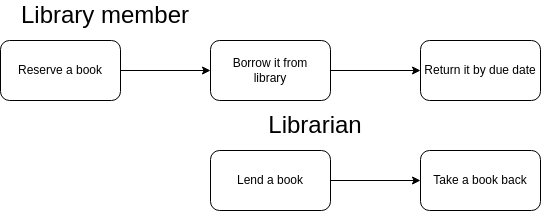
\includegraphics[scale=.75]{../drawio/Jibrarian-Main-Process.drawio.png}
    \centering
\end{figure}

\pagebreak
\section{Navigation}
\begin{figure}[!ht]
    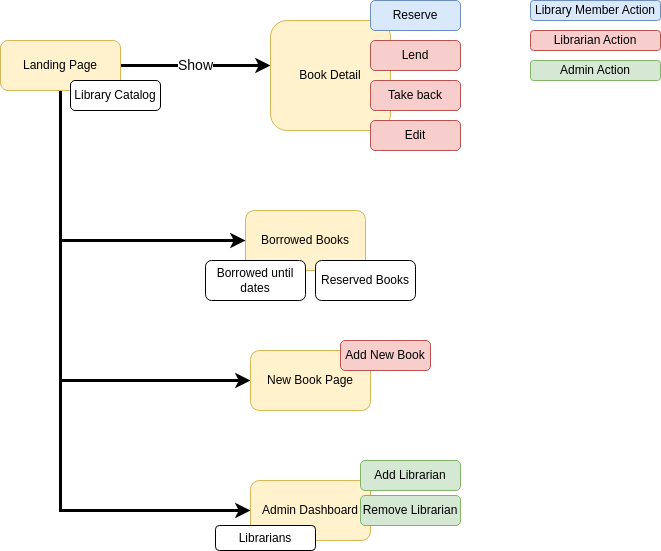
\includegraphics[scale=.7]{../drawio/Jibrarian-Navigation.drawio.png}
    \centering
\end{figure}

\pagebreak
\section{Mockups}

\subsection*{Library Member}

\begin{figure}[!ht]
    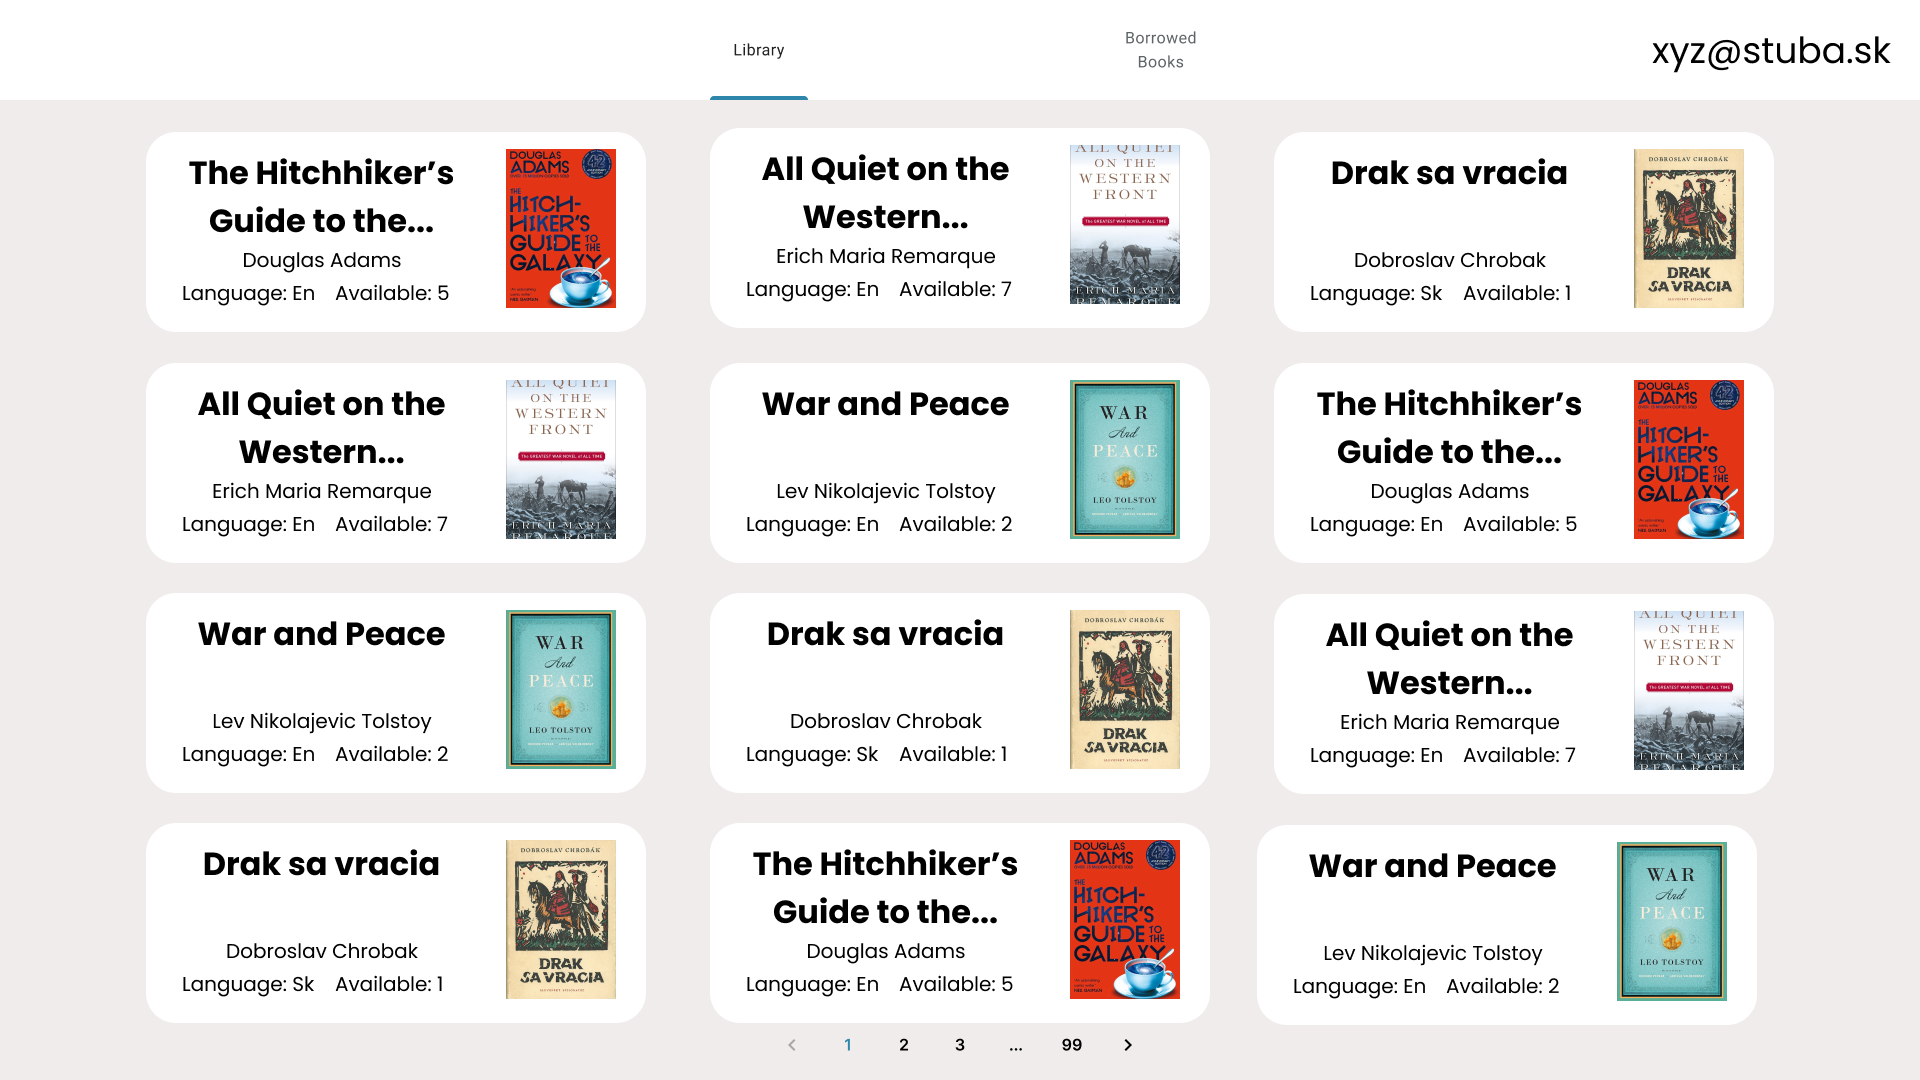
\includegraphics[scale=.2]{../mockups/Landing-page.png}
    \centering
    \caption{Landing page}
\end{figure}

\begin{figure}[!ht]
    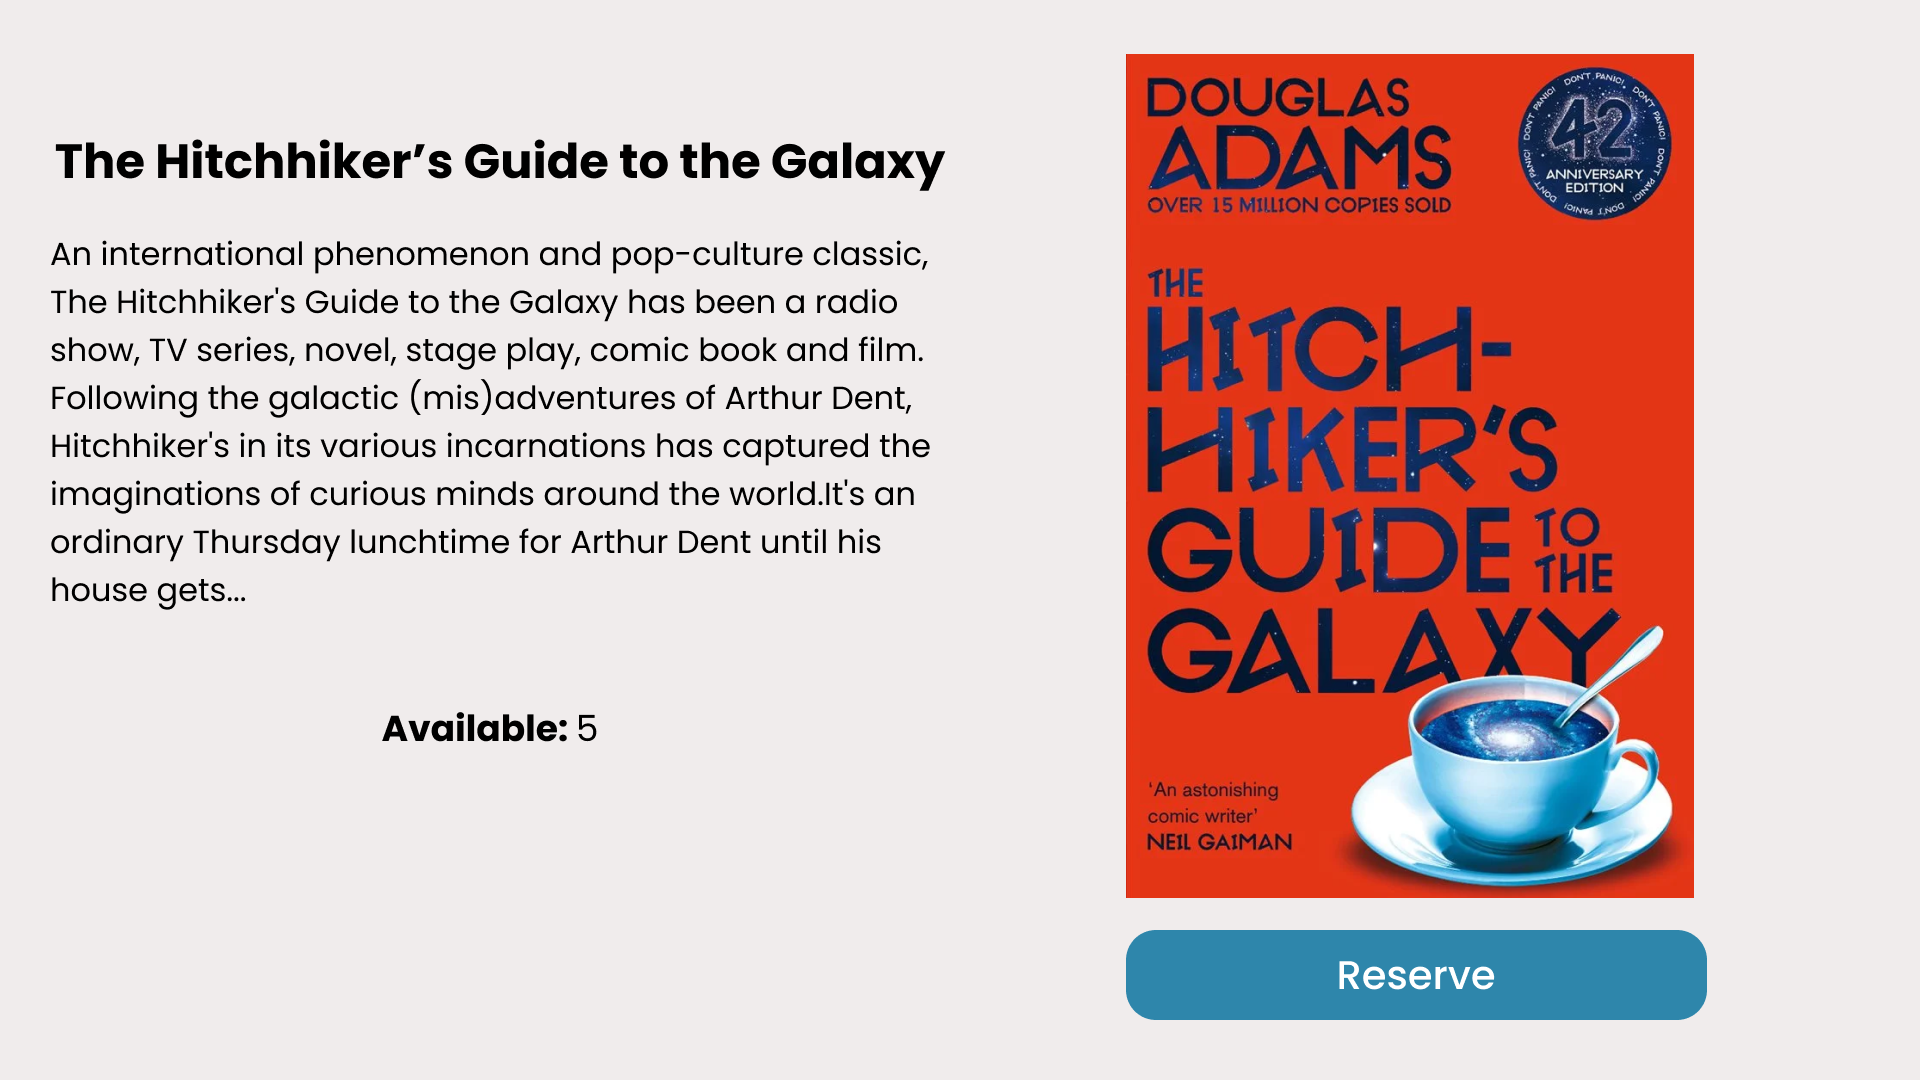
\includegraphics[scale=.2]{../mockups/Book-detail-Modal.png}
    \centering
    \caption{Book detail modal}
\end{figure}

\begin{figure}[!ht]
    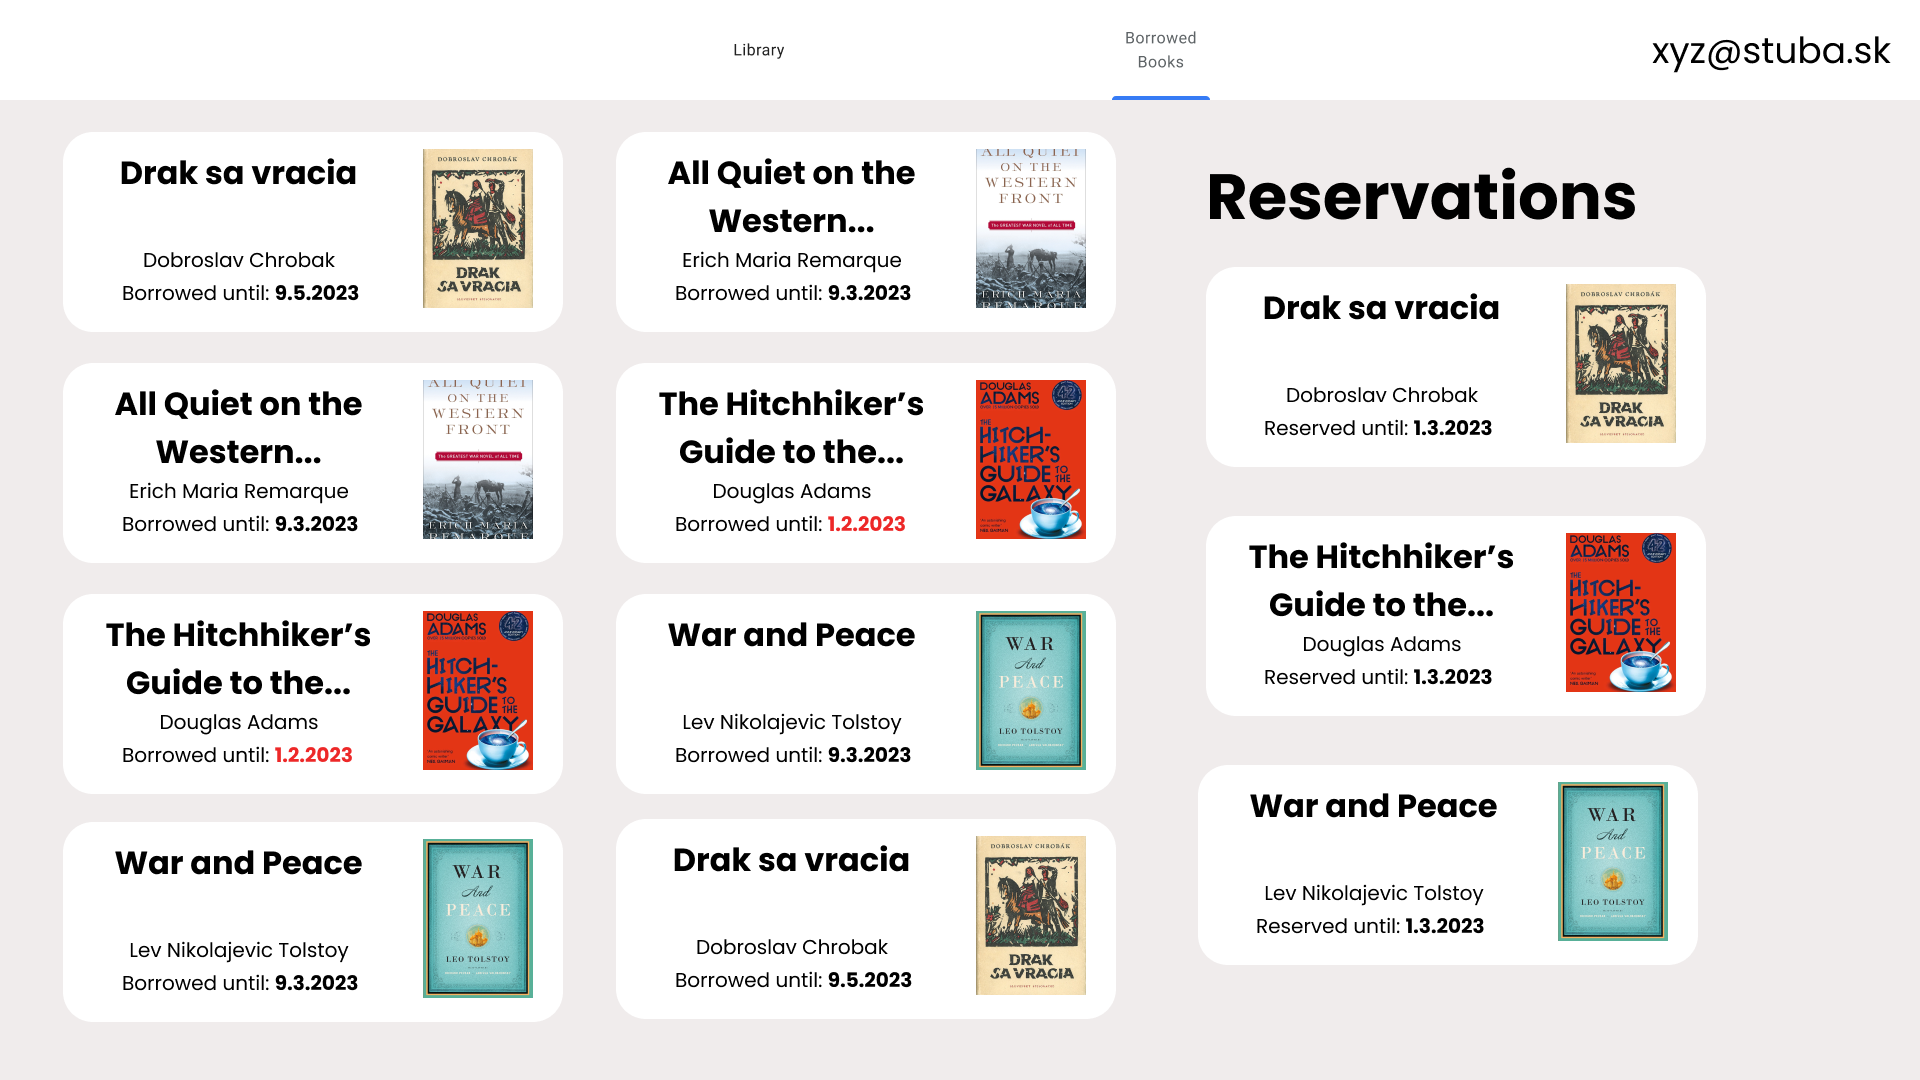
\includegraphics[scale=.2]{../mockups/Borrowed-books-Page.png}
    \centering
    \caption{Borrowed books page}
\end{figure}

\subsection*{Librarian}

\begin{figure}[!ht]
    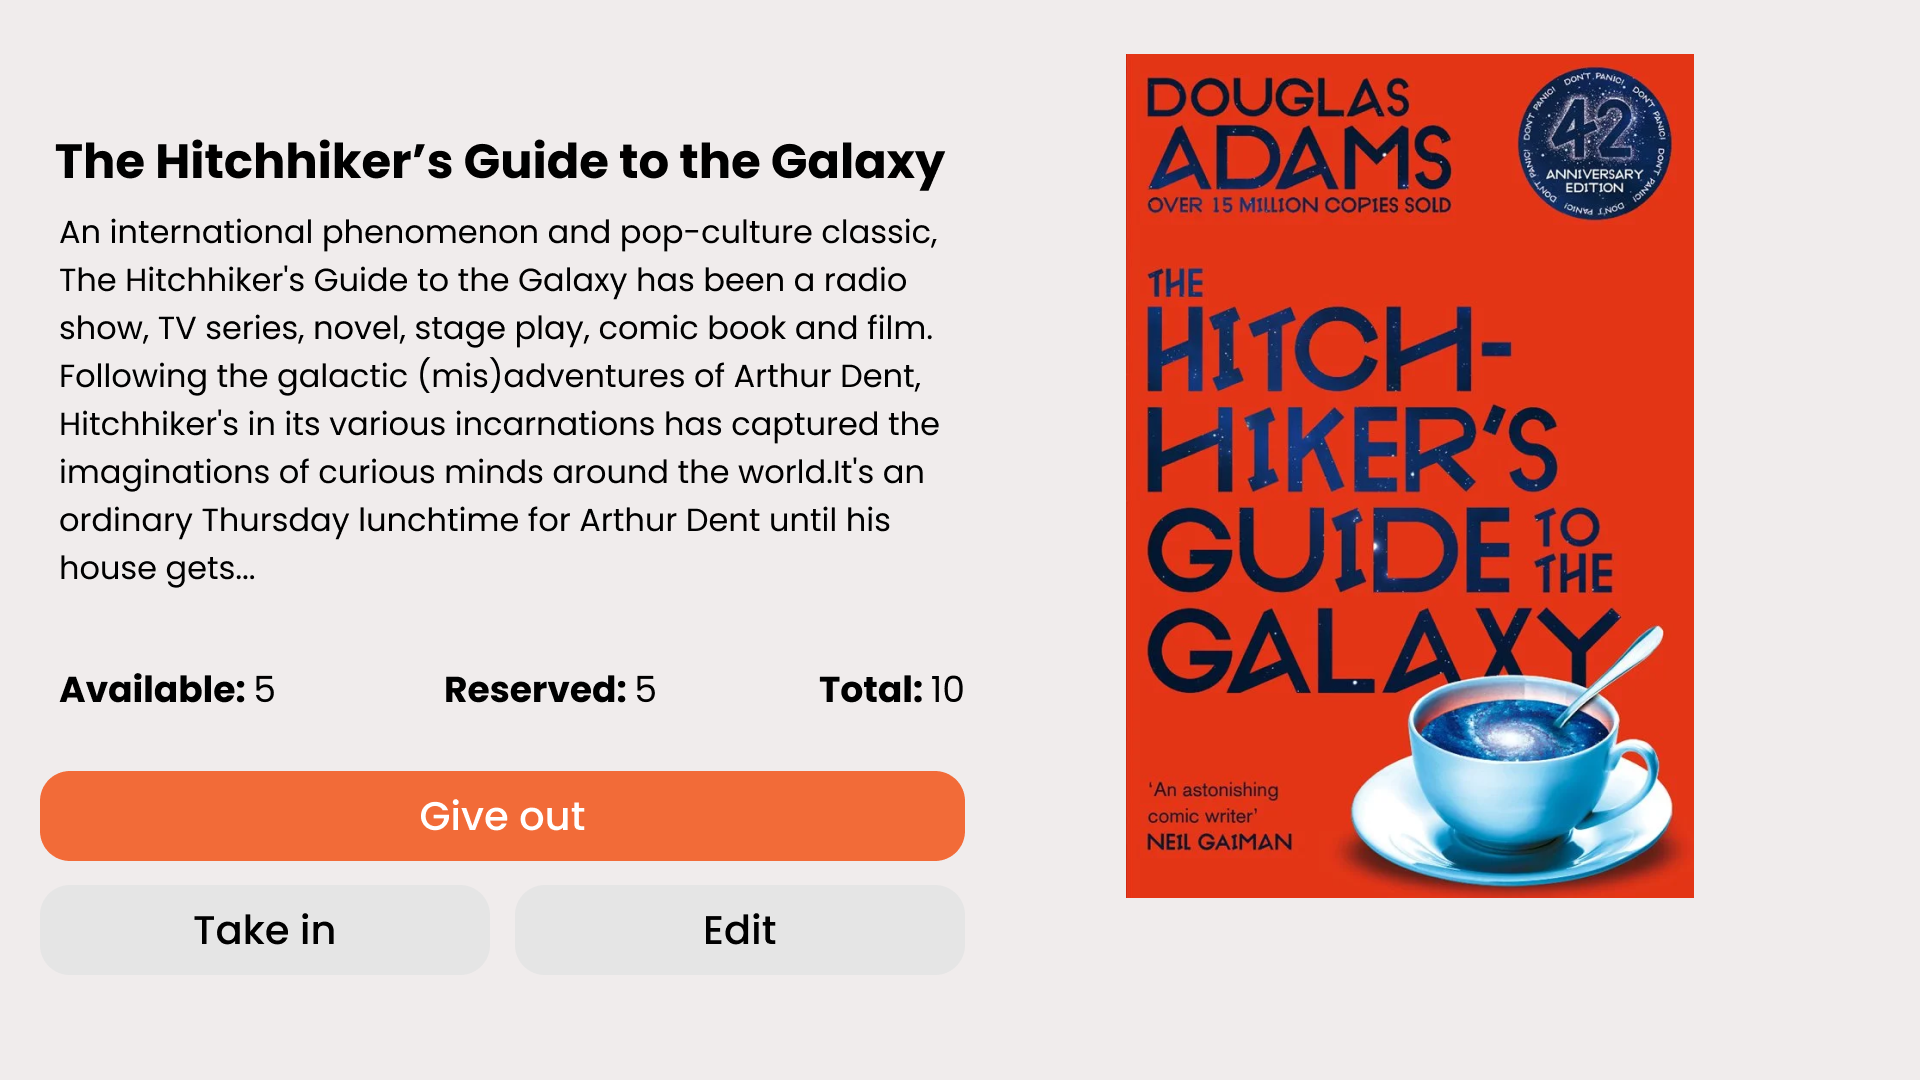
\includegraphics[scale=.2]{../mockups/Librarian-book-detail-Modal.png}
    \centering
    \caption{Book detail modal}
\end{figure}

\begin{figure}[!ht]
    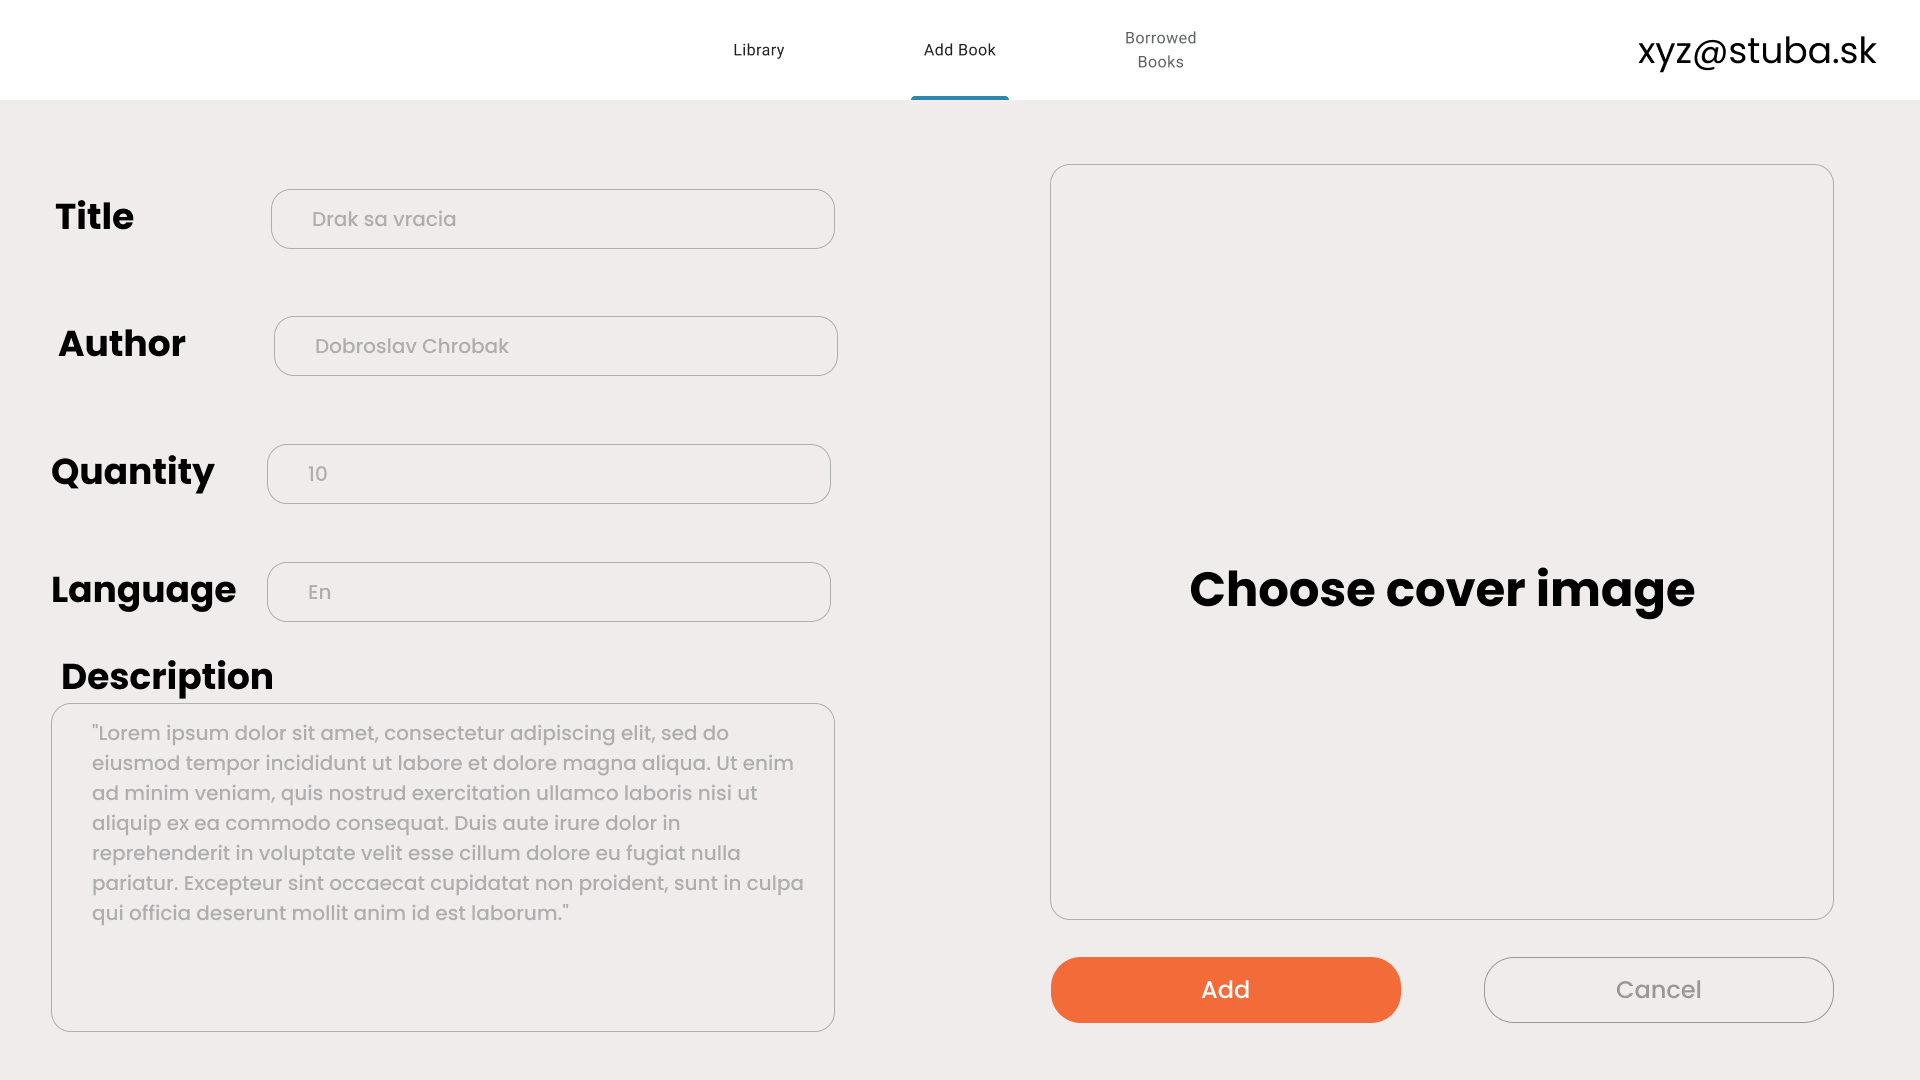
\includegraphics[scale=.2]{../mockups/Add-book-Page.png}
    \centering
    \caption{Add Book page}
\end{figure}

\pagebreak
\subsection*{Administrator}

\begin{figure}[!ht]
    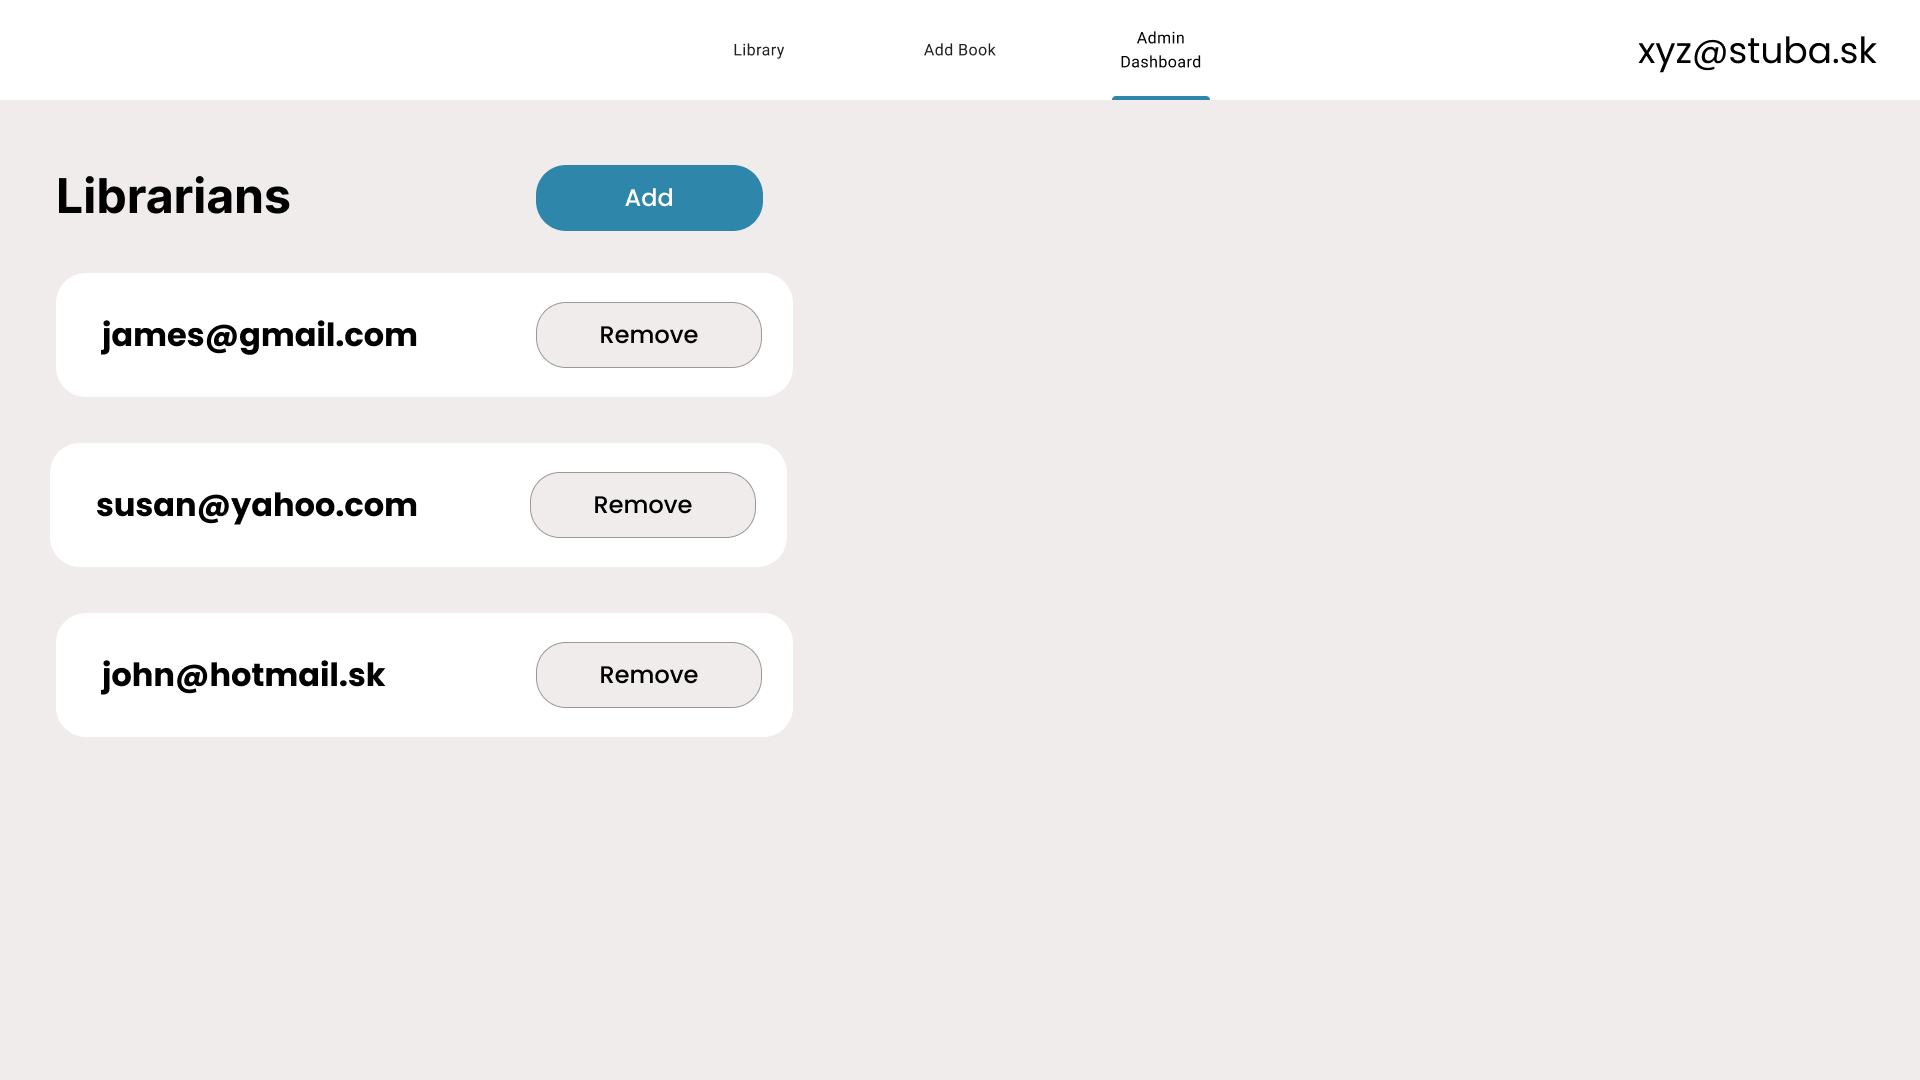
\includegraphics[scale=.2]{../mockups/Admin-dashboard.png}
    \centering
    \caption{Admin dashboard}
\end{figure}

\section{Non-functional requirements}

\begin{enumerate}
    \item Platforms: This application is made for desktop. It's developed in Java. Runnable on Windows and Linux.
    \item Usability: The application should be easy to interact with. It should have a nice clear layout, that for example even older people could use.
    \item Scalability: application should be able to be used by several users at the same time without any performance loss.
    \item Performance: this application should be able to run on even older hardware efficiently without using too many resources.
\end{enumerate}

\section{ArchiMate Diagrams}

This section contains exported diagrams from \emph{doc/eea/vava-jibrarian.qea}
Enterprise Architect file. For better details, please open referenced file
in Enterprise Architect.

\pagebreak
\subsection{Organization Viewpoint}
\begin{figure}[!ht]
    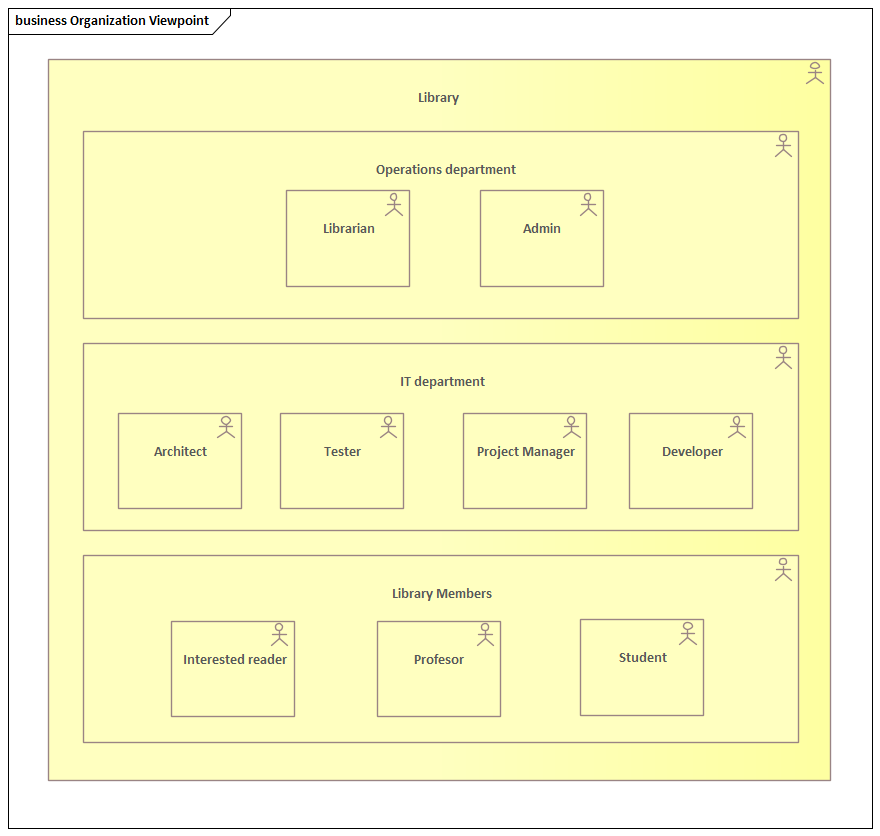
\includegraphics[scale=.9]{../ea/Organization Viewpoint.png}
    \centering
\end{figure}

\pagebreak
\subsection{Business Process Cooperation}
\begin{figure}[!ht]
    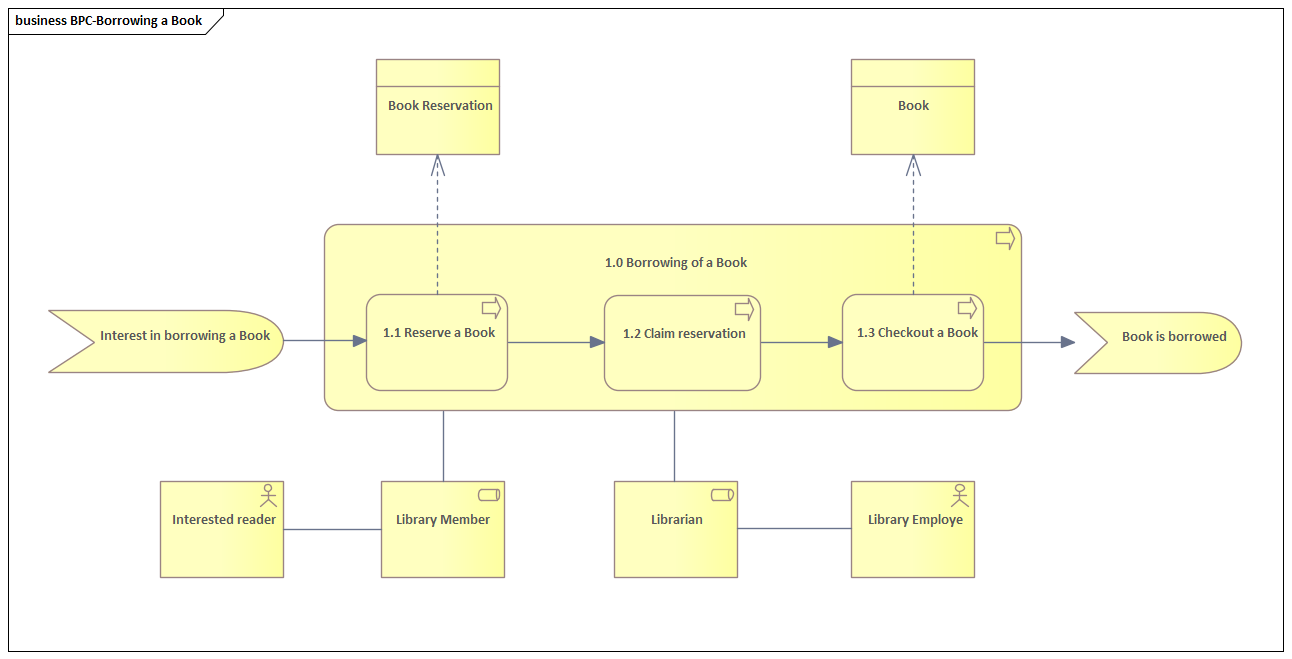
\includegraphics[scale=.65]{../ea/BPC-Borrowing a Book.png}
    \centering
\end{figure}

\pagebreak
\subsection{Product viewpoint}
\begin{figure}[!ht]
    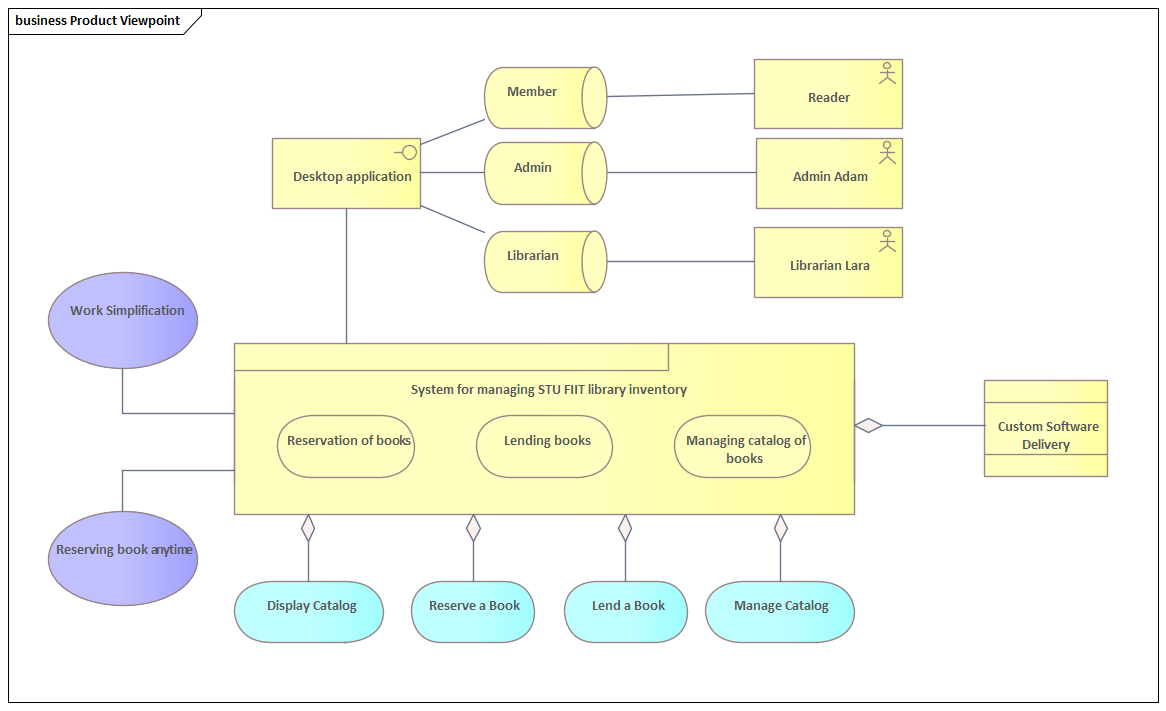
\includegraphics[scale=.7]{../ea/Product Viewpoint.png}
    \centering
\end{figure}

\pagebreak
\subsection{Application Cooperation Viewpoint}
\begin{figure}[!ht]
    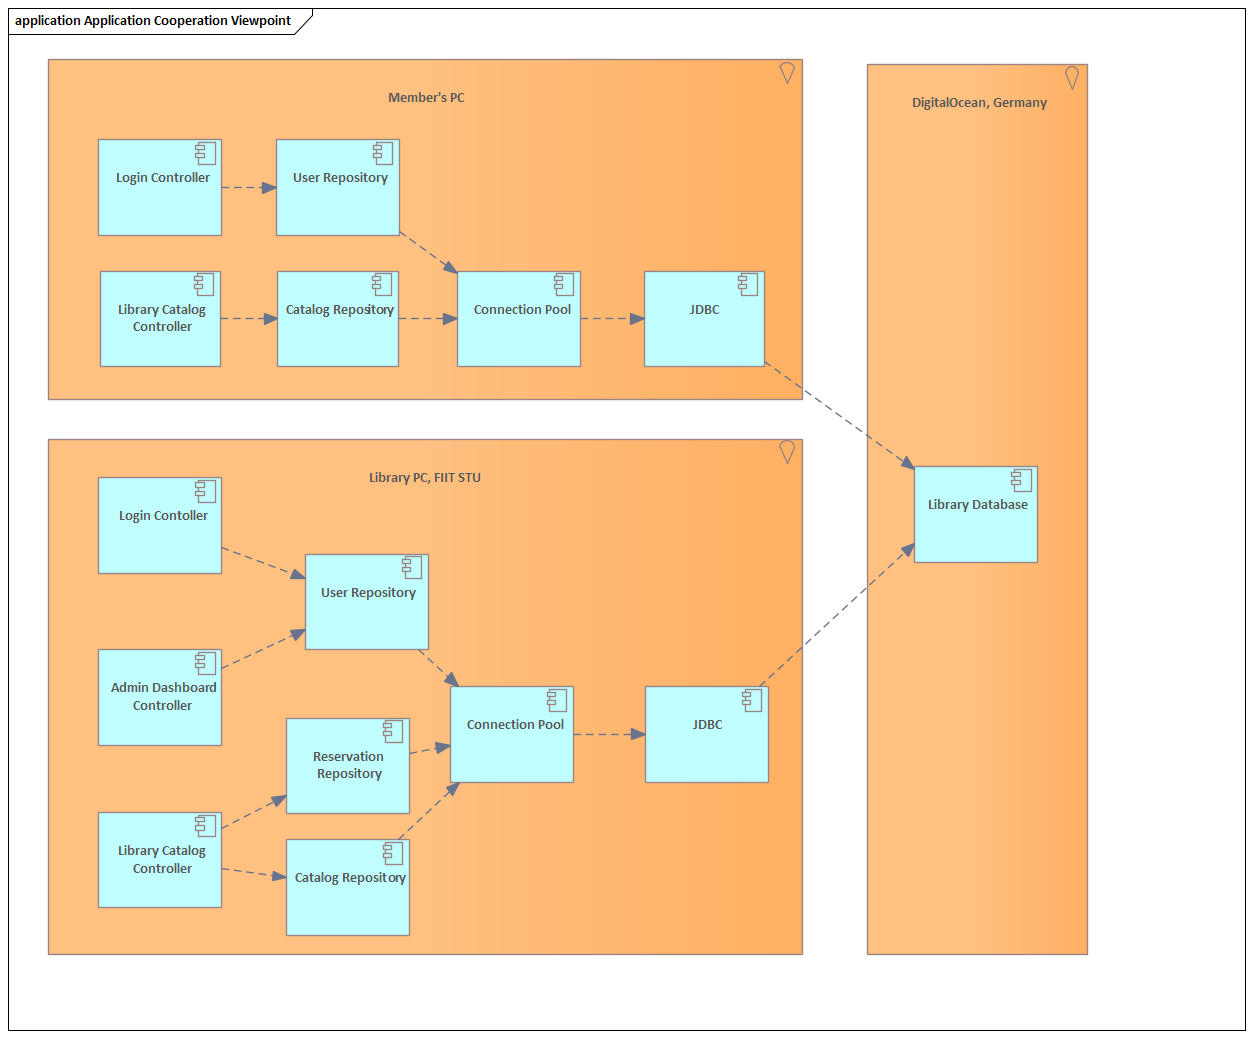
\includegraphics[scale=.6]{../ea/Application Cooperation Viewpoint.png}
    \centering
\end{figure}

\pagebreak
\subsection{Technology Viewpoint}
\begin{figure}[!ht]
    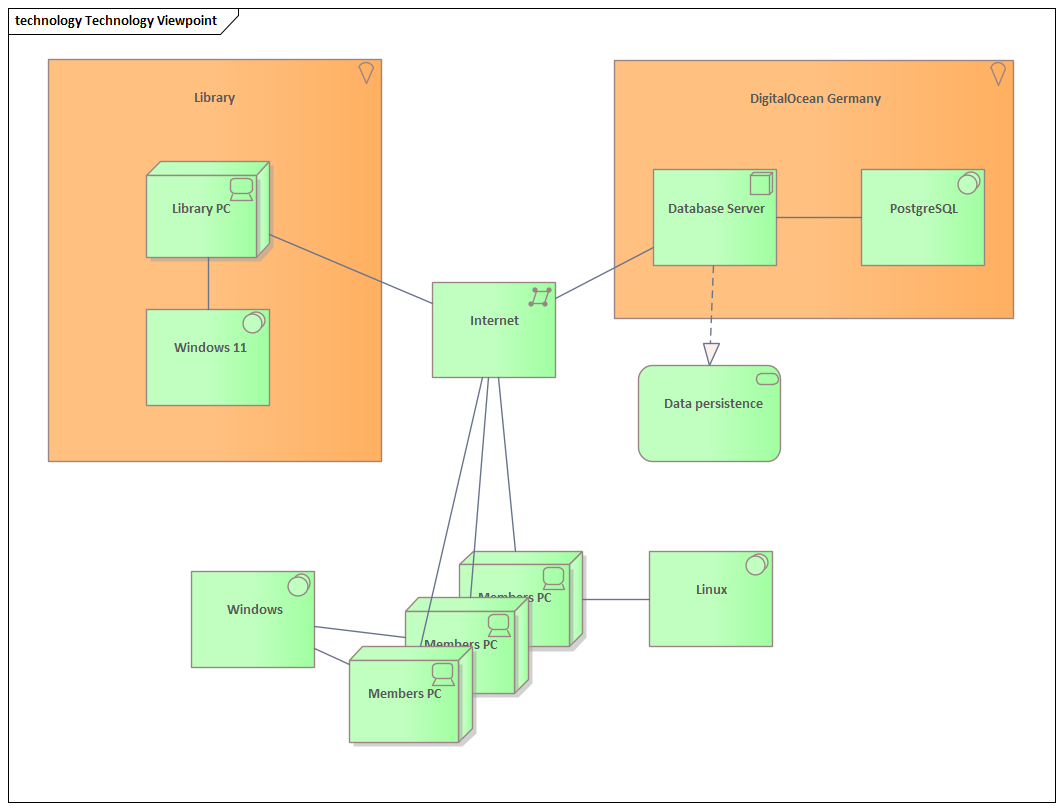
\includegraphics[scale=.8]{../ea/Technology Viewpoint.png}
    \centering
\end{figure}

\pagebreak
\subsection{Layered Viewpoint}
\begin{figure}[!ht]
    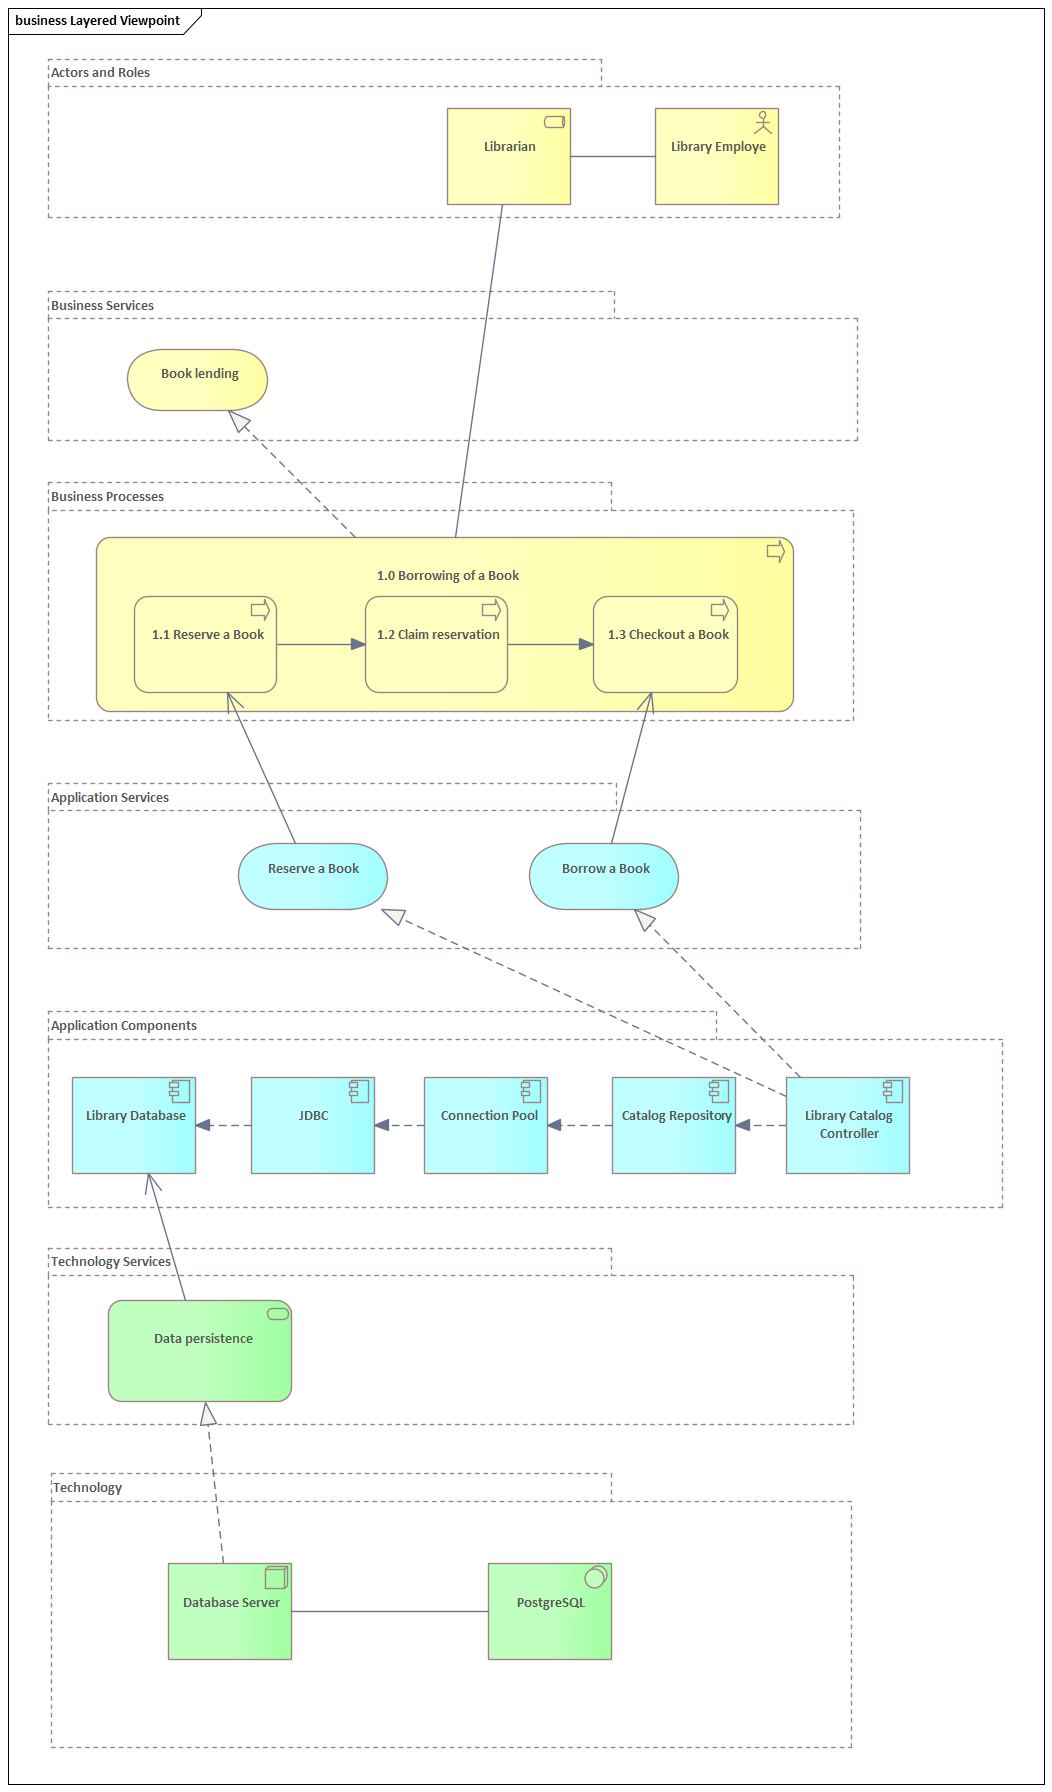
\includegraphics[scale=.5]{../ea/Layered Viewpoint.png}
    \centering
\end{figure}

\section{Class Diagram}

Class diagram is too big to be included in this documentation (if included, it would
be unreadable). In this section there are only parts of the whole class diagram.
To view the whole class diagram, please open the \emph{doc/eea/vava-jibrarian.qea}
in Enterprise Architect and see the \emph{Class Diagram} model.

\subsection{Package sk.fiit.jibrarian.model}

This part shows main classes serving as a model for Jibrarian application.

\begin{figure}[!ht]
    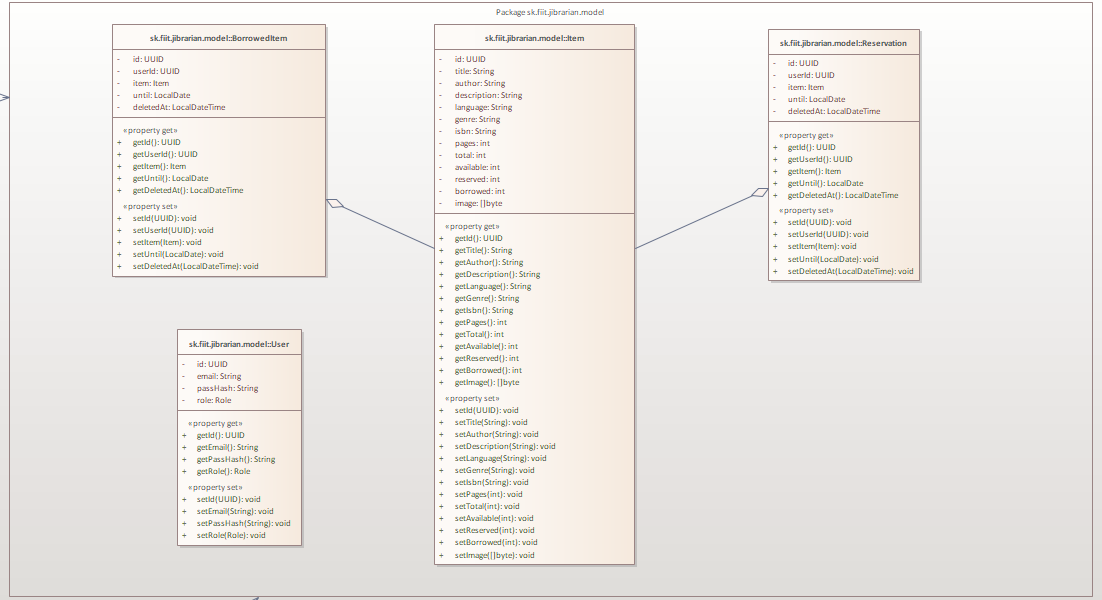
\includegraphics[scale=.5]{../ea/Class Diagram model.png}
    \centering
\end{figure}

\subsection{Package sk.fiit.jibrarian.data}

This part of class diagram documents the class hierarchy of the
\textbf{sk.fiit.jibrarian.data} package, which is responsible for reading and
writing data of the application to either RAM or database (based on run environment).

\begin{figure}[!ht]
    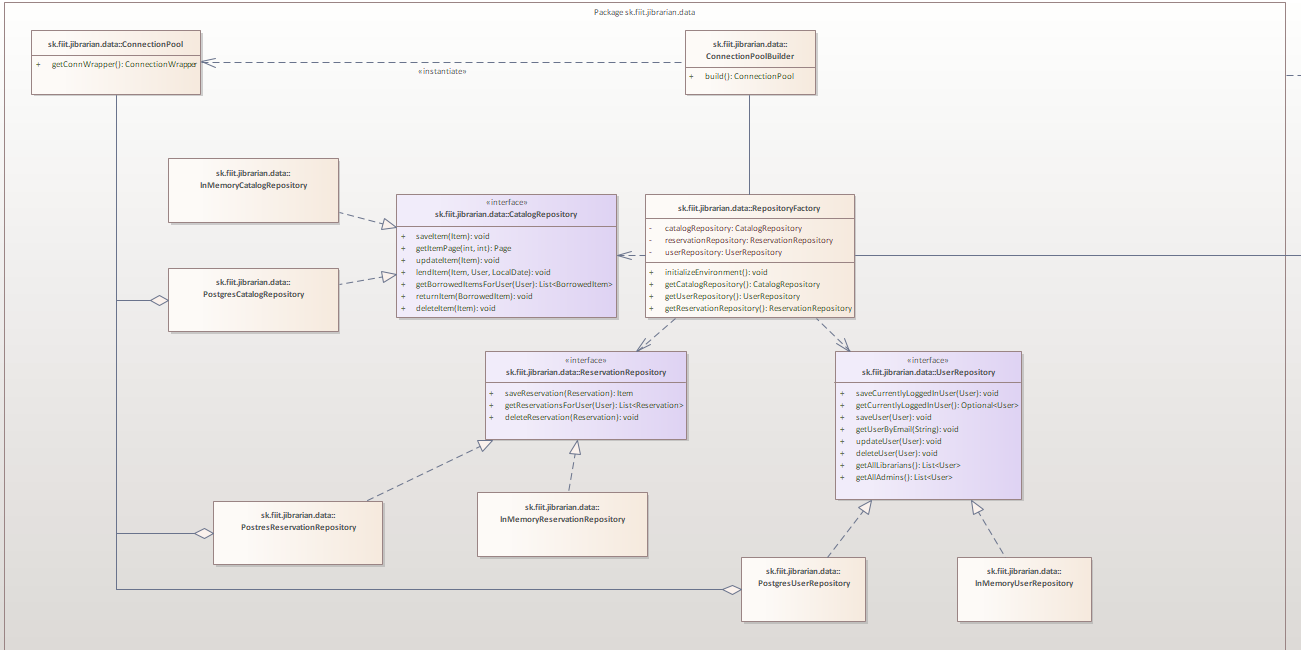
\includegraphics[scale=.35]{../ea/Class Diagram data.png}
    \centering
\end{figure}

\pagebreak
\subsection{Package sk.fiit.jibrarian.controllers}

This part of class diagram shows all JavaFx controllers used in GUI part of Jibrarian.

\begin{figure}[!ht]
    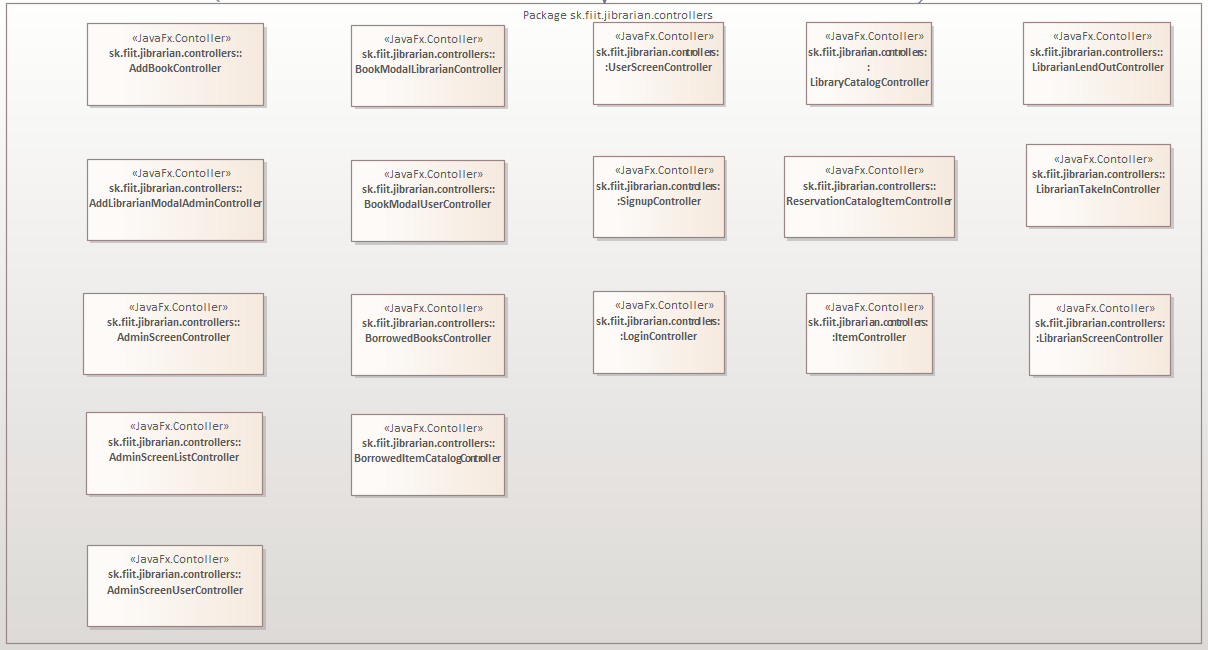
\includegraphics[scale=.4]{../ea/Class Diagram controllers.png}
    \centering
\end{figure}

\pagebreak
\section{Assignment requirements}

List below documents how are different assignment requirements fulfilled
\begin{enumerate}
    \item Collections: usage of List\textless T\textgreater and ArrayList\textless
          T\textgreater
    \item Logging: logs containing information about user flow, data manipulation,
          exceptions and malfunctions
    \item Localization: application can be run in English, or Slovak language
    \item XML: logs are also stored into xml file
    \item Regular Expressions: email validation is done with a regular expression
    \item JDBC: application connects to a PostgreSQL DBMS and read/writes data to it
    \item Validation: SQL injections are prevented with use of prepared statements
    \item GUI: user interface is written in JavaFX
    \item 3 types of users: application contains functionality for Library Members, Librarians and Admins
    \item Encapsulation in all classes
\end{enumerate}

\section{Used technology}

This application is written in Java 17 and uses Maven (version 3.8.7) build
system for building and testing.

\subsection*{Dependencies}

Dependencies listed below are taken from projects \emph{pom.xml}.

\begin{itemize}
    \item JavaFx
          \begin{itemize}
              \item org.openjfx:javafx-controls:19.0.2.1
              \item org.openjfx:javafx-fxml:19.0.2.1
          \end{itemize}
    \item PostgreSQL driver: org.postgresql:postgresql:42.6.0
    \item JUnit
          \begin{itemize}
              \item org.junit.jupiter:junit-jupiter:5.9.2
              \item org.junit.jupiter:junit-jupiter-engine:5.9.2
          \end{itemize}
    \item BCrypt: at.favre.lib:bcrypt:0.10.2
\end{itemize}

\section{How to run}

The easiest way to run the application is importing it into Intellij IDE, and
using provided Maven run configurations. More can be read in \emph{./doc/setup.md}
and \emph{./doc/run.md}

Provided jar file is a fat jar with all dependencies included.

\section{What did we learn}

At the start of this summer term, we had no clue about how projects are built
in the real world. Until now we had little experience with building something
in a team and a more real environment.

From organizational standpoint we have experienced on our own skin how hard it
can be to organize a team of 5 programmers. We saw how valuable Jira is for
tracking what needs to be done and how far have we come. Weekly meetings were
really helpful to show the whole team how we are progressing together, who is
working on what and for sharing newly learned knowledge. Also we learned
importance of communication the hard way. We can't count how many times someone
wrote a piece of code, which was reviewed and seemed fine, but introduced
a bug in other part of code.

Other lesson we learned is that writing code isn't enough in the real world.
Concepts as enterprise architecture and design are important and should be well
thought out, because otherwise there will be problems when the code is already
written, but doesn't do anything useful in context of a project.

Each of us learned new Java programming concepts, which can also be used in
different languages. Such as logging and importance of what to log and not,
how to customize software so it can be used in different locations. How does
connecting and communicating with database work. How to program GUI in JavaFX
and other smaller concepts, but still important.

Even though our project isn't the greatest application, isn't written in
the best way possible, we still learned a lot and all five of us did everything
we could to build Jibrarian to the best of our abilities.

We want to express our gratitude to our teacher Mr. Reiter, for teaching us a lot
of important and useful things.


\end{document}